\documentclass[11pt]{scrartcl}

\usepackage[sexy]{evan}
\usepackage{microtype}
\microtypesetup{expansion=false}
\usepackage{pgfplots}
\pgfplotsset{compat=1.15}
\usepackage{mathrsfs}
\usetikzlibrary{arrows}
\usepackage{graphics}
\usepackage{listings}
\usepackage{tikz}
\usepackage{ amssymb }
\usepackage[dvipsnames]{xcolor}
\definecolor{red1}{RGB}{255, 153, 153}
\definecolor{green1}{RGB}{204, 255, 204}
\definecolor{blue1}{RGB}{204, 255, 255}
\definecolor{yellow1}{RGB}{255, 247, 160}

\definecolor{red2}{RGB}{255, 102, 102}
\definecolor{green2}{RGB}{108, 255, 108}
\definecolor{blue2}{RGB}{94, 204, 255}
\definecolor{yellow2}{RGB}{255, 250, 104}

\definecolor{red2.5}{RGB}{255,76,76}
\definecolor{green2.5}{RGB}{54, 247, 54}
\definecolor{blue2.5}{RGB}{51, 189, 255}
\definecolor{yellow2.5}{RGB}{255, 242, 52}


\definecolor{red3}{RGB}{255, 51, 51}
\definecolor{green3}{RGB}{0, 240, 0}
\definecolor{blue3}{RGB}{9, 175, 255}
\definecolor{yellow3}{RGB}{255, 234, 0}

\definecolor{red3.5}{RGB}{229, 25, 25}
\definecolor{green3.5}{RGB}{0, 194, 0}
\definecolor{blue3.5}{RGB}{4, 143, 209}
\definecolor{yellow3.5}{RGB}{255,220,0}

\definecolor{red4}{RGB}{204, 0, 0}
\definecolor{green4}{RGB}{0, 149, 0}
\definecolor{blue4}{RGB}{0, 111, 164}
\definecolor{yellow4}{RGB}{255, 206, 0}

\newcommand{\camod}[1]{\frac{\ZZ}{#1 \ZZ}}
\newcommand{\modm}[1]{\text{ mod } #1}
\newcommand{\campm}[1]{\frac{\ZZ}{m\ZZ}}
\newcommand{\paren}[1]{\left(  #1 \right)}
\newcommand{\proc}[1]{Esto va a aparecer si no procrastino :S (Procrastinando desde #1)}


\title{ME CORTAN EN ENERO }
\subtitle{PONTE A ENTRENAR}
\author{Emmanuel Buenrostro}


\begin{document}

\maketitle

\section{Problemas}
\begin{problem}[Cono Sur 2016/6]
We say that three different integers are friendly if one of them divides the product of the other two. Let $n$ be a positive integer.

a) Show that, between $n^2$ and $n^2+n$, exclusive, does not exist any triplet of friendly numbers.

b) Determine if for each $n$ exists a triplet of friendly numbers between $n^2$ and $n^2+n+3\sqrt{n}$ , exclusive.
\end{problem}
\begin{problem}[Israel 2023/6]
Determine if there exists a set $S$ of $5783$ different real numbers with the following property:
For every $a,b\in S$ (not necessarily distinct) there are $c\neq d$ in $S$ so that $a\cdot b=c+d$.
\end{problem}
\begin{problem}[USAMO 2022/2]
    	Let $b\geq2$ and $w\geq2$ be fixed integers, and $n=b+w$. Given are $2b$ identical black rods and $2w$ identical white rods, each of side length 1.

We assemble a regular $2n-$gon using these rods so that parallel sides are the same color. Then, a convex $2b$-gon $B$ is formed by translating the black rods, and a convex $2w$-gon $W$ is formed by translating the white rods. An example of one way of doing the assembly when $b=3$ and $w=2$ is shown below, as well as the resulting polygons $B$ and $W$.

\begin{center}
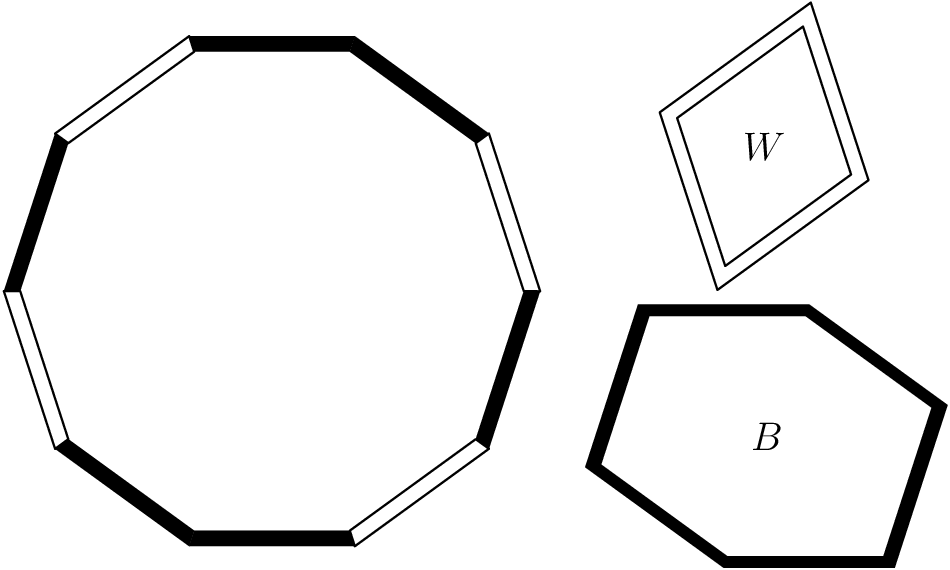
\includegraphics[scale=0.5]{USAMO2022_2.png}
\end{center}
Prove that the difference of the areas of $B$ and $W$ depends only on the numbers $b$ and $w$, and not on how the $2n$-gon was assembled.
\end{problem}
\begin{problem}[AC ABC387F]
\url{https://atcoder.jp/contests/abc387/tasks/abc387_f}
\end{problem}
\begin{problem}[Rioplatense 2024/3.5]
    Let $S = \{2, 3, 4, \dots\}$ be the set of positive integers greater than 1. Find all functions $f : S \to S$ that satisfy
\[
\text{gcd}(a, f(b)) \cdot \text{lcm}(f(a), b) = f(ab)
\]for all pairs of integers $a, b \in S$.

Clarification: $\text{gcd}(a,b)$ is the greatest common divisor of $a$ and $b$, and $\text{lcm}(a,b)$ is the least common multiple of $a$ and $b$.
\end{problem}
\begin{problem}[India 2024/5]
Let points $A_1$, $A_2$ and $A_3$ lie on the circle $\Gamma$ in a counter-clockwise order, and let $P$ be a point in the same plane. For $i \in \{1,2,3\}$, let $\tau_i$ denote the counter-clockwise rotation of the plane centred at $A_i$, where the angle of rotation is equial to the angle at vertex $A_i$ in $\triangle A_1A_2A_3$. Further, define $P_i$ to be the point $\tau_{i+2}(\tau_{i}(\tau_{i+1}(P)))$, where the indices are taken modulo $3$ (i.e., $\tau_4 = \tau_1$ and $\tau_5 = \tau_2$).

Prove that the radius of the circumcircle of $\triangle P_1P_2P_3$ is at most the radius of $\Gamma$.
\end{problem}
\begin{problem}[Entrenas Nacionales 2025 Grupo 1/ 15. Principio Extremo / 12]
Se tiene un número finito de polígonos en el plano (no necesariamente convexo) de forma que cualesquiera dos polígonos del conjunto se intersectan. Prueba que existe una línea que intersecta a todos los polígonos.
\end{problem}
\begin{problem}[OMM 2018/6]
    Encuentra todos los enteros $n\geq 3$ tales que existe un polígono convexto de $n$ lados $A_1A_2\dots A_n$ que tenga las siguientes características:
 \begin{itemize} 
 \item  Todos los ángulos internos de $A_1A_2\dots A_n$ son iguales. 
 \item  No todos los lados de $A_1A_2\dots A_n$ son iguales.
 \item  Existe un triángulo $T$ y un punto $O$ en el interior de $A_1A_2\dots A_n$ tal que los $n$ triángulos $OA_1A_2, OA_2A_3,\dots OA_nA_1$ son todos semejantes a $T$.
\end{problem}
\begin{problem}[OTIS Russian Combo Russia 2014/9.1]
  Each lattice point of $\ZZ^2$ is colored with one of three colors,
  with every color used at least once.
  Show that one can find a right triangle with pairwise distinct colored vertices.
\end{problem}
\begin{problem}[Vietnam National Olympiad for High School Student 2022/12]
Given Fibonacci sequence $(F_n),$ and a positive integer $m$, denote $k(m)$ by the smallest positive integer satisfying $F_{n+k(m)}\equiv F_n(\bmod m),$ for all natural numbers $n$.
a) Prove that: For all $m_1,m_2\in \mathbb{Z^+}$, we have:$$k([m_1,m_2])=[k(m_1),k(m_2)].$$(Here $[a,b]$ is the least common multiple of $a,b.$)

b) Determine $k(2),k(4),k(5),k(10).$
\end{problem}
\begin{problem}[OTIS Orders Romania TST 1996]
Find all primes $ p,q $ such that $ \alpha^{3pq} -\alpha \equiv 0 \pmod {3pq} $ for all integers $ \alpha $.
\end{problem}
\begin{problem}[Entrenas Nacionales 2025 Grupo 1/ 13.Puntos Variables Mapeos Proyectivos / 11]
En el triangulo $ABC$, el $\angle B$ es obtuso y $AB \neq BC$. Sea $\omega$ el circuncirculo de $ABC$ y $O$ su circuncentro. $N$ es el punto medio del arco $ABC$. El circuncirculo de $BON$ interseca a $AC$ en puntos $X$ y $Y$. Sean $P$ y $Q$ puntos distintos de $B$ las intersecciones de $BX$ y $BY$ con $\omega$ respectivamente. Demuestra que $P,Q$ y la reflexion de $N$ respecto a la recta $AC$ son colineares.  
\end{problem}
\begin{problem}[Canada 2023/3]
    An acute triangle is a triangle that has all angles less than $90^{\circ}$ ($90^{\circ}$ is a Right Angle). Let $ABC$ be an acute triangle with altitudes $AD$, $BE$, and $CF$ meeting at $H$. The circle passing through points $D$, $E$, and $F$ meets $AD$, $BE$, and $CF$ again at $X$, $Y$, and $Z$ respectively. Prove the following inequality:$$\frac{AH}{DX}+\frac{BH}{EY}+\frac{CH}{FZ} \geq 3.$$
\end{problem}
\begin{problem}[Leer/Aprender Cauchy]
Leer/Aprender Cauchy
\end{problem}
\begin{problem}[Bulgaria JBMO TST 2023/2]
Let $x, y,$ and $z$ be positive real numbers such that $xy + yz + zx = 3$. Prove that
$$\frac{x + 3}{y + z} + \frac{y + 3}{z + x} + \frac{z + 3}{x + y} + 3 \ge 27 \cdot \frac{(\sqrt{x} + \sqrt{y} + \sqrt{z})^2}{(x + y + z)^3}.$$
\end{problem}
\begin{problem}[The A-Schwaat Line]
  Let $ABC$ be a triangle with altitude $\ol{AD}$.
  Let $M$ and $N$ denote the midpoints of $\ol{AD}$ and $\ol{BC}$.
  Show that line $MN$ passes through
  the symmedian point of $\triangle ABC$
  (this line is called the $A$-Schwatt line).
\end{problem}
\begin{problem}[IMO SL 2022/C4]
Let $n > 3$ be a positive integer. Suppose that $n$ children are arranged in a circle, and $n$ coins are distributed between them (some children may have no coins). At every step, a child with at least 2 coins may give 1 coin to each of their immediate neighbors on the right and left. Determine all initial distributions of the coins from which it is possible that, after a finite number of steps, each child has exactly one coin.  
\end{problem}
\begin{problem}[Argentina Ibero TST 2016/2]
Let $ABCD$ be a trapezoid with bases $BC \parallel AD$ and non-parallel sides $AB$ and $CD$. On the diagonals $AC$ and $BD$, let $P$ and $Q$ be the points such that $AC$ bisects $\angle BPD$ and $BD$ bisects $\angle AQC$. Prove that $\angle BPD = \angle AQC$.
\end{problem}
\begin{problem}[Iran TST 2015/3.2]
Assume that $a_1, a_2, a_3$ are three given positive integers consider the following sequence:
$a_{n+1}=\text{lcm}[a_n, a_{n-1}]-\text{lcm}[a_{n-1}, a_{n-2}]$ for $n\ge 3$
Prove that there exist a positive integer $k$ such that $k\le a_3+4$ and $a_k\le 0$.
($[a, b]$ means the least positive integer such that$ a\mid[a,b], b\mid[a, b]$ also because $\text{lcm}[a, b]$ takes only nonzero integers this sequence is defined until we find a zero number in the sequence)
\end{problem}
\begin{problem}[DIME 2022/11]
A positive integer $n$ is called $\textit{un-two}$ if there does not exist an ordered triple of integers $(a,b,c)$ such that exactly two of$$\dfrac{7a+b}{n},\;\dfrac{7b+c}{n},\;\dfrac{7c+a}{n}$$are integers. Find the sum of all un-two positive integers.
\end{problem}
\begin{problem}[Malaysian APMO Camp Selection Test 2023/1]
For which $n\ge 3$ does there exist positive integers $a_1<a_2<\cdots <a_n$, such that:$$a_n=a_1+...+a_{n-1}, \hspace{0.5cm} \frac{1}{a_1}=\frac{1}{a_2}+...+\frac{1}{a_n}$$are both true?
\end{problem}
\begin{problem}[Entrenas Nacionales 2025 Grupo 1 /11. Razon Cruzada y Armonicos / 17]
Sea $ABC$ un triangulo con incentro $I$ y sea $D$ el punto de tangencia de su incirculo con $BC$. Sean $X,Y$ puntos en el segmento $BI,CI$ respectivamente, tal que $\angle BAC=2\angle XAY$. Prueba que $\angle XDY=90$. 
\end{problem}
\begin{problem}[Turkey EGMO TST 2024/6]
Let $\omega_1$ and $\omega_2$ be two different circles that intersect at two different points, $X$ and $Y$. Let lines $l_1$ and $l_2$ be common tangent lines of these circles such that $l_1$ is tangent $\omega_1$ at $A$ and $\omega_2$ at $C$ and $l_2$ is tangent $\omega_1$ at $B$ and $\omega_2$ at $D$. Let $Z$ be the reflection of $Y$ respect to $l_1$ and let $BC$ and $\omega_1$ meet at $K$ for the second time. Let $AD$ and $\omega_2$ meet at $L$ for the second time. Prove that the line tangent to $\omega_1$ and passes through $K$ and the line tangent to $\omega_2$ and passes through $L$ meet on the line $XZ$.
\end{problem}
\begin{problem}[Sudafrica 2012/6]
   Find all functions $f:\mathbb{N}\to\mathbb{R}$ such that
$f(km)+f(kn)-f(k)f(mn)\ge 1$
for all $k,m,n\in\mathbb{N}$.
\end{problem}
\begin{problem}[JBMO 2024/4]
  Three friends Archie, Billie, and Charlie play a game. At the beginning of the game, each of them has a pile of $2024$ pebbles. Archie makes the first move, Billie makes the second, Charlie makes the third and they continue to make moves in the same order. In each move, the player making the move must choose a positive integer $n$ greater than any previously chosen number by any player, take $2n$ pebbles from his pile and distribute them equally to the other two players. If a player cannot make a move, the game ends and that player loses the game.
$\hspace{5px}$ Determine all the players who have a strategy such that, regardless of how the other two players play, they will not lose the game.
\end{problem}
\begin{problem}[Euler Olympiad 2023/R1.8]
	Let $a$, $b$, $c$, and $d$ be positive integers such that the following two inequalities hold: $a < 10^{20} \cdot c$ and $b > 10^{23} \cdot d$.
Determine the minimum possible value of the total number of positive integer pairs $(n, m)$ for which $n \cdot m = 2^{2023}$ and

$$ \frac {ab}{n} + \frac{cd}{m} < \frac{(a + c)(b + d)}{n + m}$$
\end{problem}
\begin{problem}[Iran TST 2023/1.5]
Suppose that $n\ge2$ and $a_1,a_2,...,a_n$ are natural numbers that $ (a_1,a_2,...,a_n)=1$. Find all strictly increasing function $f: \mathbb{Z}  \to \mathbb{R} $ that:

$$ \forall  x_1,x_2,...,x_n \in  \mathbb{Z} :       f(\sum_{i=1}^{n} {x_ia_i}) = \sum_{i=1}^{n} {f(x_ia_i})$$
\end{problem}
\begin{problem}[EGMO 2024/1]
Two different integers $u$ and $v$ are written on a board. We perform a sequence of steps. At each step we do one of the following two operations:

(i) If $a$ and $b$ are different integers on the board, then we can write $a + b$ on the board, if it is not
already there.
(ii) If $a$, $b$ and $c$ are three different integers on the board, and if an integer $x$ satisfies $ax^2 +bx+c = 0$,
then we can write $x$ on the board, if it is not already there.

Determine all pairs of starting numbers $(u, v)$ from which any integer can eventually be written on the board after a finite sequence of steps.
\end{problem}
\begin{problem}[USA TST 2025/2]
Let $a_1, a_2, \dots$ and $b_1, b_2, \dots$ be sequences of real numbers for which $a_1 > b_1$ and
\begin{align*}
    a_{n+1} &= a_n^2 - 2b_n\\
    b_{n+1} &= b_n^2 - 2a_n
\end{align*}for all positive integers $n$. Prove that $a_1, a_2, \dots$ is eventually increasing (that is, there exists a positive integer $N$ for which $a_k < a_{k+1}$ for all $k > N$).
\end{problem}
\begin{problem}[OTIS Orders Don Zagier]
Let $S$ denote the integers $n\ge 2$ with the property that for any positive integer $a$ we have$$a^{n+1} \equiv a \pmod n.$$Show that $S$ is finite and determine its elements.
\end{problem}
\begin{problem}[PAGMO 2021/6]
   Let $ABC$ be a triangle with incenter $I$, and $A$-excenter $\Gamma$. Let $A_1,B_1,C_1$ be the points of tangency of $\Gamma$ with $BC,AC$ and $AB$, respectively. Suppose $IA_1, IB_1$ and $IC_1$ intersect $\Gamma$ for the second time at points $A_2,B_2,C_2$, respectively. $M$ is the midpoint of segment $AA_1$. If the intersection of $A_1B_1$ and $A_2B_2$ is $X$, and the intersection of $A_1C_1$ and $A_2C_2$ is $Y$, prove that $MX=MY$.
\end{problem}
\begin{problem}[EGMO 2024/4]
	For a sequence $a_1<a_2<\cdots<a_n$ of integers, a pair $(a_i,a_j)$ with $1\leq i<j\leq n$ is called interesting if there exists a pair $(a_k,a_l)$ of integers with $1\leq k<l\leq n$ such that$$\frac{a_l-a_k}{a_j-a_i}=2.$$For each $n\geq 3$, find the largest possible number of interesting pairs in a sequence of length $n$.
\end{problem}
\begin{problem}[USACO 2016 JAN BRZ 2]
\url{https://usaco.org/index.php?page=viewproblem2&cpid=592}
\end{problem}
\begin{problem}[JBMOSL 2021/C4]
Alice and Bob play a game together as a team on a $100 \times 100$ board with all unit squares initially white. Alice sets up the game by coloring exactly $k$ of the unit squares red at the beginning. After that, a legal move for Bob is to choose a row or column with at least $10$ red squares and color all of the remaining squares in it red. What is the
smallest $k$ such that Alice can set up a game in such a way that Bob can color the entire board red after finitely many moves?
\end{problem}
\begin{problem}[OTIS Orders HMMT November 2014]
Determine all positive integers $1 \le m \le 50$ for which there exists an integer $n$ for which $m$ divides $n^{n+1}+1$.
\end{problem}
\begin{problem}[CF 2052J]
\url{https://codeforces.com/problemset/problem/2052/J}
\end{problem}
\begin{problem}[AC ARC80A]
\url{https://atcoder.jp/contests/abc069/tasks/arc080_a?lang=en}
\end{problem}
\begin{problem}[USA TST 2015/1]
  (Walkthrough OTIS)
  Let $ABC$ be a scalene triangle with incenter $I$ whose incircle is
  tangent to $\ol{BC}$, $\ol{CA}$, $\ol{AB}$ at $D$, $E$, $F$,
  respectively.  Denote by $M$ the midpoint of $\ol{BC}$ and
  let $P$ be a point in the interior of $\triangle ABC$
  so that $MD = MP$ and $\angle PAB = \angle PAC$.
  Let $Q$ be a point on the incircle such that $\angle AQD = 90^{\circ}$.
  Prove that either $\angle PQE = 90^{\circ}$ or $\angle PQF = 90^{\circ}$.
\end{problem}
\begin{problem}[IOI 2023 LONGEST TRIP]
\url{https://oj.uz/problem/view/IOI23_longesttrip}
\end{problem}
\begin{problem}[Entrenas Nacionales 2025 Grupo 1/ 14.Doble Conteo / 3.8]
Sea $n$ un numero entero mayor que 1. Para un entero positivo $m$, sea $S_m=\{ 1,2,\ldots ,mn \}.$ Supongamos que existe un conjunto de $2n$ elementos $T$ tal que 
\begin{itemize}
\item cada elemento de $T$ es un subconjunto de $S_m$ con $m$ elementos
\item cada par de elementos en $T$ comparte como maximo un elemento comun
\item cada elemento de $S_m$ esta contenido exactamente en dos elementos de $T$
\end{itemize}
Determina el valor maximo posible de $m$ en terminos de $n$.
\end{problem}
\begin{problem}[AC ABC388E]
\url{https://atcoder.jp/contests/abc388/tasks/abc388_e}
\end{problem}
\begin{problem}[OTIS Funcionales Indian Postal Set 2016]
  Determine all functions $f \colon \RR \to \RR$ satisfying
  \[ f\left( xf(y)-yf(x) \right) = f(xy)-xy \]
  for all real numbers $x$ and $y$.

\end{problem}
\begin{problem}[AC ABC385E]
\url{https://atcoder.jp/contests/abc385/tasks/abc385_e}
\end{problem}
\begin{problem}[AC ABC387E]
\url{https://atcoder.jp/contests/abc387/tasks/abc387_e}
\end{problem}

\end{document}
